\documentclass[,hyphens]{sigchi}

% Use this section to set the ACM copyright statement (e.g. for
% preprints).  Consult the conference website for the camera-ready
% copyright statement.

% Copyright
\CopyrightYear{2020}
%\setcopyright{acmcopyright}
\setcopyright{acmlicensed}
%\setcopyright{rightsretained}
%\setcopyright{usgov}
%\setcopyright{usgovmixed}
%\setcopyright{cagov}
%\setcopyright{cagovmixed}
% DOI
\doi{https://doi.org/10.1145/3313831.XXXXXXX}
% ISBN
\isbn{978-1-4503-6708-0/20/04}
%Conference
\conferenceinfo{CHI'20,}{April  25--30, 2020, Honolulu, HI, USA}
%Price
\acmPrice{\$15.00}

% Use this command to override the default ACM copyright statement
% (e.g. for preprints).  Consult the conference website for the
% camera-ready copyright statement.

%% HOW TO OVERRIDE THE DEFAULT COPYRIGHT STRIP --
%% Please note you need to make sure the copy for your specific
%% license is used here!
% \toappear{
% Permission to make digital or hard copies of all or part of this work
% for personal or classroom use is granted without fee provided that
% copies are not made or distributed for profit or commercial advantage
% and that copies bear this notice and the full citation on the first
% page. Copyrights for components of this work owned by others than ACM
% must be honored. Abstracting with credit is permitted. To copy
% otherwise, or republish, to post on servers or to redistribute to
% lists, requires prior specific permission and/or a fee. Request
% permissions from \href{mailto:Permissions@acm.org}{Permissions@acm.org}. \\
% \emph{CHI '16},  May 07--12, 2016, San Jose, CA, USA \\
% ACM xxx-x-xxxx-xxxx-x/xx/xx\ldots \$15.00 \\
% DOI: \url{http://dx.doi.org/xx.xxxx/xxxxxxx.xxxxxxx}
% }

% Arabic page numbers for submission.  Remove this line to eliminate
% page numbers for the camera ready copy
\pagenumbering{arabic}

% Load basic packages
\usepackage{balance}       % to better equalize the last page
\usepackage{graphics}      % for EPS, load graphicx instead 
\usepackage[T1]{fontenc}   % for umlauts and other diaeresis
\usepackage{txfonts}
\usepackage{mathptmx}
\usepackage[pdflang={en-US},pdftex]{hyperref}
\usepackage{color}
\usepackage{booktabs}
\usepackage{textcomp}

% Some optional stuff you might like/need.
\usepackage{microtype}        % Improved Tracking and Kerning
% \usepackage[all]{hypcap}    % Fixes bug in hyperref caption linking
\usepackage{ccicons}          % Cite your images correctly!
% \usepackage[utf8]{inputenc} % for a UTF8 editor only

% If you want to use todo notes, marginpars etc. during creation of
% your draft document, you have to enable the "chi_draft" option for
% the document class. To do this, change the very first line to:
% "\documentclass[chi_draft]{sigchi}". You can then place todo notes
% by using the "\todo{...}"  command. Make sure to disable the draft
% option again before submitting your final document.
\usepackage{todonotes}

% Paper metadata (use plain text, for PDF inclusion and later
% re-using, if desired).  Use \emtpyauthor when submitting for review
% so you remain anonymous.
\def\plaintitle{SIGCHI Conference Proceedings Format}
\def\plainauthor{First Author, Second Author, Third Author,
  Fourth Author, Fifth Author, Sixth Author}
\def\emptyauthor{}
\def\plainkeywords{Authors' choice; of terms; separated; by
  semicolons; include commas, within terms only; this section is required.}
\def\plaingeneralterms{Documentation, Standardization}

% llt: Define a global style for URLs, rather that the default one
\makeatletter
\def\url@leostyle{%
  \@ifundefined{selectfont}{
    \def\UrlFont{\sf}
  }{
    \def\UrlFont{\small\bf\ttfamily}
  }}
\makeatother
\urlstyle{leo}

% To make various LaTeX processors do the right thing with page size.
\def\pprw{8.5in}
\def\pprh{11in}
\special{papersize=\pprw,\pprh}
\setlength{\paperwidth}{\pprw}
\setlength{\paperheight}{\pprh}
\setlength{\pdfpagewidth}{\pprw}
\setlength{\pdfpageheight}{\pprh}

% Make sure hyperref comes last of your loaded packages, to give it a
% fighting chance of not being over-written, since its job is to
% redefine many LaTeX commands.
\definecolor{linkColor}{RGB}{6,125,233}
\hypersetup{%
  pdftitle={\plaintitle},
% Use \plainauthor for final version.
%  pdfauthor={\plainauthor},
  pdfauthor={\emptyauthor},
  pdfkeywords={\plainkeywords},
  pdfdisplaydoctitle=true, % For Accessibility
  bookmarksnumbered,
  pdfstartview={FitH},
  colorlinks,
  citecolor=black,
  filecolor=black,
  linkcolor=black,
  urlcolor=linkColor,
  breaklinks=true,
  hypertexnames=false
}

% create a shortcut to typeset table headings
% \newcommand\tabhead[1]{\small\textbf{#1}}

% End of preamble. Here it comes the document.
\begin{document}

\title{We are the Greatest Showmen: Configuring Mobile Learning Technologies for Student-Led Activities}

\numberofauthors{3}
\author{%
  \alignauthor{Leave Authors Anonymous\\
    \affaddr{for Submission}\\
    \affaddr{City, Country}\\
    \email{e-mail address}}\\
  \alignauthor{Leave Authors Anonymous\\
    \affaddr{for Submission}\\
    \affaddr{City, Country}\\
    \email{e-mail address}}\\
  \alignauthor{Leave Authors Anonymous\\
    \affaddr{for Submission}\\
    \affaddr{City, Country}\\
    \email{e-mail address}}\\
}

\maketitle

\begin{abstract}
While the use of mobile learning technologies by teachers and community experts has been explored by HCI research, little attention has been given to how they could be used by students to enhance project-based learning processes. Following an action research approach, we report on engagements inside and outside of the classroom with both teachers and students from three different UK schools, using a variety of configurations of project-based, mobile learning to work within given time constraints to produce student-led mobile learning activities using the OurPlace application. We also report on the use of the OurPlace to facilitate an exchange of knowledge and values between a class from an ethnically diverse inner-city school and the children of a community of travelling Showmen. We contribute insights gained from these studies, including the effects of compromise in response to given contextual constraints, how mobile technologies can harness students' existing desire for independence and how they can be configured to surface and leverage local heritage as a learning resource.
\end{abstract}


% ACM Classfication

\begin{CCSXML}
<ccs2012>
<concept>
<concept_id>10003120.10003121</concept_id>
<concept_desc>Human-centered computing~Human computer interaction (HCI)</concept_desc>
<concept_significance>500</concept_significance>
</concept>
<concept>
<concept_id>10003120.10003121.10003125.10011752</concept_id>
<concept_desc>Human-centered computing~Haptic devices</concept_desc>
<concept_significance>300</concept_significance>
</concept>
<concept>
<concept_id>10003120.10003121.10003122.10003334</concept_id>
<concept_desc>Human-centered computing~User studies</concept_desc>
<concept_significance>100</concept_significance>
</concept>
</ccs2012>
\end{CCSXML}

\ccsdesc[500]{Human-centered computing~Human computer interaction (HCI)}
\ccsdesc[300]{Human-centered computing~Haptic devices}
\ccsdesc[100]{Human-centered computing~User studies}

% Author Keywords
\keywords{\plainkeywords}

% Print the classification codes
\printccsdesc
Please use the 2012 Classifiers and see this link to embed them in the text: \url{https://dl.acm.org/ccs/ccs_flat.cfm}



\section{Introduction}

Blumenfeld et al. lament that small, easily assessed tasks which focus on low-level facts and skills (i.e. tasks commonly found on worksheets) have become the focus of many classrooms \cite{Blumenfeld1991}. They argue that these tasks afford students `\textit{few opportunities to represent knowledge in a variety of ways, pose and solve real problems, or use their knowledge to create artifacts}'. Arguably this can be at least partly attributed to pressures and limitations put upon teachers and schools, as they work within structures which expect them to conform to quantifiable testing methods, propagating the aforementioned worksheet-style tasks and `teaching to the test'. The head of the UK's Office for Standards in Education (Ofsted) has noted that `\textit{[Ofsted] have created a situation where second-guessing the test can trump the pursuit of real, deep knowledge and understanding}' \cite{Ofsted2018}. Blumenfeld et al. argue that a preferable alternative is project-based learning (PBL), which they describe as an approach to teaching and learning which focuses on engaging students through the investigation of non-trivial, `authentic' problems in a manner which supports learner autonomy over the course of an extended project. However, the restrictions placed upon teachers frequently impacts their time affordances, curriculum content and pedagogical approaches. This has meant that implementing project-based learning in UK schools has proven to be a challenge \cite{TheEducationEndowmentFoundation2016}.

At the same time, mobile learning (`\textit{learning across multiple contexts, through social and content interactions using personal electronic devices}' \cite{Crompton2013}, AKA `m-learning') has grown to play a large role within schools in the UK, with ready access to tablet computers becoming more common in schools (44\% of UK schools are expected to have one tablet per child by 2020 \cite{BritishEducationalSuppliersAssociation2015}), and their general ubiquity meaning most of the younger population is familiar with their use (87\% of UK adults report owning a smartphone \cite{Statistica2018}, as do 84\% of children aged between 8-16 \cite{Statistica2018a}). Despite this, there is a lack of HCI research around how mobile learning technologies can play a role in the PBL process \cite{Chan2015}.

In this paper, we contribute insights from studies held with three different UK schools and a summer school of Travelling Showmen, each having their own social contexts and teaching restrictions. We report on the creation of a PBL curriculum designed around the open-source mobile application OurPlace, the deployment of it in these contexts and the effects of re-configuring the curriculum to meet contextual challenges. We introduce `project-based mobile learning', and discuss how this process can harness students' existing desires for independence as a motivational force, offer new avenues for leveraging local heritage as a learning resource, and give an example of how mobile learning technologies can benefit project-based learning processes.

\section{Related Work}
In this section we briefly introduce and discuss the purported benefits of constructionism and project-based learning, and how mobile learning technologies can fit into the PBL process.

\subsection{Constructionism}
The learning theory of constructionism, introduced by Seymour Papert in the mid-1980s, argues that constructing, sharing and reflecting upon physical or virtual `public entities' can be a powerful way for learners to build `knowledge structures'--collections of knowledge, concepts and facts interrelated through various semantic relationships \cite{PapertSeymourandHarel1991a}. Papert argues that the process of learning is the building of these knowledge structures, a process which--while it occurs irrespective of the circumstances of the learning--happens `\textit{especially felicitously in a context where the learner is consciously engaged in constructing a public entity}'. These public entities could range from physical artefacts such as models of buildings, virtual programming code or even conceptual theories of the universe. 

In their overview of constructionism, Noss and Hoyles argue that constructionist working environments offer a medium in which learners can `\textit{explore and learn from feedback, much as one can master a foreign language by living in the appropriate country}' \cite{Noss2017}. Noss and Hoyles also claim that they afford learners to take ownership of a construction-based approach, potentially leading to greater engagement, confidence and empowerment. Finally, they posit that through exploration and construction of public entities, learners can encounter `powerful ideas': `\textit{concepts and strategies  that confront and build upon intuitive knowledge}'. For this reason, Noss and Hoyles argue that constructionist tools need to be expressive enough to facilitate these ideas emerging through the learner's construction of public entities.

\subsection{Project-Based Learning}
Project-based learning approaches present learners with a given `problem' or task, requiring them to investigate around and work on a given subject over a longer period of time. These problems are non-trivial and often framed as `authentic', in that they are somewhat applicable to the real world \cite{Blumenfeld1991}. Frequently, students' projects will result in the creation of an artifact in response to the given problem (such as videos, reports, artworks, websites or performances \cite{Holubova2008}), in effect making PBL a method of applying constructionism in response to real-world problems and supporting the inclusion of prior knowledge, domain research and greater levels of student autonomy. It's worth noting that several other configurations of PBL have been developed over time (e.g. problem-based learning), however they mostly conform to the same essential elements: a challenging problem or question; sustained inquiry; an element of authenticity; a degree of student control; reflection; critique and revision; and a final public product \cite{Larmer2015}. Previous research has argued that these projects can serve to build bridges between classroom activities and real-life experiences \cite{Blumenfeld1991}, enhance applied and conceptual knowledge around a subject \cite{Boaler1999}, and that greater levels of autonomy and challenge can result in higher levels of student engagement \cite{Wurdinger2007}.

Project-based learning is also recognised as fertile ground for technology-enhanced learning. Bell argues that `\textit{technology as a means, not an end, enables students to experiment with different technologies for all aspects of PBL}' (including research and data collection, knowledge sharing and artifact creation) and that it can be `\textit{highly engaging to students, because it taps into their fluency with computers}' \cite{Bell2010}. ChanLin describes how students used digital technologies within PBL for researching on the web, taking photographs, participating in online communities and creating web pages as final artifacts \cite{ChanLin2008}. Krajcik et al note that while the use of mobile and desktop technologies help students build knowledge structures and form deeper and richer understandings of the subjects at hand, teachers frequently run into challenges in gaining access to computing hardware due to multiple classes sharing resources \cite{Krajcik2006}.

While some studies have found that project-based instruction is not necessarily more demanding in terms of teaching time and resources \cite{Al-Balushi2014}, Blumenfeld et al posit that by its nature PBL `\textit{requires active engagement of students' effort over an extended period of time}' \cite{Blumenfeld1991}. Krajcik et al argue that `\textit{it takes more time to complete a task where students are constructing their own knowledge in meaningful, situated activities}', leading to teachers being hesitant to put it into practice when faced with strict and competing curriculum goals \cite{Krajcik2006}. The non-profit organisation Innovation Unit note `\textit{[PBL] can be a powerful learning strategy if it is part of a whole school change process, and [schools] are ready and able to make the necessary time and staff available}' \cite{InnovationUnit2016}, suggesting that putting PBL into practice requires substantial changes in how teachers approach classroom structures, activities and tasks. This is easier said than done, thanks to governmental pressures and restrictions frequently placed upon UK teachers, often limiting the amount of time they can dedicate to particular topics and experiential learning methodologies which don't target given examinations (particularly in later school years, which place greater emphasis on quantifiable assessment) \cite{Ofsted2018}.

\subsection{Mobile Learning}
The adoption of mobile devices into UK classrooms has been dramatic, with nearly half of UK schools being expected to have one tablet per child within the next few years \cite{BritishEducationalSuppliersAssociation2015}. While traditional desktop and laptop devices are currently still more common in schools (numbering approximately 3.4 million in 2017 \cite{BritishEducationalSuppliersAssociation2017}), mobile devices have been touted as having a number of advantages over their more stationary counterparts: for example, Traxler argues that mobile technologies can offer structured educational experiences which can be situated in--and responsive to--authentic learning environments \cite{Traxler2011}. This makes m-learning a potentially great fit for subscribers to Lave and Wenger's Situated Learning Theory, which posits that learning unintentionally occurs in authentic activities, contexts and cultures through `legitimate participation' in communities of practice \cite{Lave1991}. Sharples et al argue that to better utilise these advantages, m-learning technologies should take into account the physical and social aspects of the learning context (both physical and social); the amount of control the learner has over the activity; and the learner's communication with others \cite{Sharples2007}.

Previous m-learning research has used these capabilities for a wide variety of applications, such as sensing tool kits to conduct citizen science \cite{Sharples2017}; enabling seamless learning across classrooms and museums on school trips \cite{Vavoula2009}; and empowering children in collecting evidence to support their advocacy and engagement in urban design processes \cite{Peacock2018}. Prior research has also shown that m-learning technologies can enhance the development of relationships with place, and act as a medium through which stakeholders can harness the underlying socioeconomic infrastructures of place as learning resources \cite{Richardson2017}. In the ParkLearn project, Richardson et al attempted to combine elements of all of the above into a single mobile application supporting creating, sharing and engaging with bespoke, place-based m-learning activities `\textit{that leverage the targeted learning environment and mobile devices' hardware to support situated learning}' \cite{Richardson2018}. Through using ParkLearn in longitudinal studies with a primary school and volunteers at a local park, the authors found that the app promoted a sense of ownership in both learners and activity creators by supporting greater degrees of creativity and independence. Furthermore, the app was shown to be an effective medium through which physical and social aspects of the local environment could be leveraged as learning resources.

Chan et al note that the use of mobile technologies in PBL has been under-researched \cite{Chan2015}. In a qualitative study with an undergraduate course, they noted that students used mobile devices for multiple stages of the PBL process, including researching the subject on the Internet, making notes, sharing materials and making use of educational applications to help understand abstract concepts. Massey et al took a different approach, presenting graduate-level students with the challenge of creating a mobile-friendly version of their course-management software, with the created software acting as the final public entity of the students' team projects \cite{Massey2006}. They argue that this pedagogical environment aimed to re-frame the students as `\textit{not only end users of mobile applications, but also as developers and decision makers}'. These studies suggest that like other forms of classroom technology, m-learning technologies can be configured to support the PBL process, or even be used to construct the project's final public entity.

\section{A Project-Based Mobile Learning Curriculum}

With this research in mind, we decided to explore how project-based m-learning  (PBML) could be effectively configured within the context of UK schools. In order to capitalise on the advantages of mobile learning technologies, we decided that any educational projects should take a situated learning approach which leveraged the schools' surrounding heritage as educational resources. As the ParkLearn application's activities were reported as being well suited to this, we believed that the construction of an activity regarding local heritage would be a good final public entity for a project. In this section we introduce the latest iteration of ParkLearn and the curriculum we created to use it as a PBML tool within UK schools.

\subsection{The OurPlace App}

OurPlace is the current iteration of the open-source ParkLearn platform, with an expanded feature set and re-branded to support its use in contexts outside of local parks \cite{Richardson2018a}. Consisting of a website and mobile applications for both Android and iOS, OurPlace supports the creation of--and sharing and engagement with--m-learning activities (`Activities'), each of which is built up from smaller, modular tasks (`Tasks'). These tasks each consist of a specific interaction (`Task Type'), which either promote creativity, emulate traditional classroom learning materials or use the device's hardware to give context-specific experiences (Table~\ref{tab:TaskTypes}). With the exception of \textit{Scan the QR Code}, all of these Task Types were present in the original ParkLearn application. OurPlace also adds support for `Follow-Up Tasks', which allow activity creators to add sub-tasks which unlock once their parent task has been completed (Figure~\ref{fig:ActivityCreation}.e). This supports the design of more complicated combinations of interactions (for example: a \textit{Location Hunt} could unlock a \textit{Record Audio} and \textit{Take a Photo} once the user arrives at a designated location).

\begin{table}
  \centering
  \begin{tabular}{l|p{50mm}}
    % \toprule
    {\small\textit{Task Type}}
    & {\small \textit{Interaction Description}} \\
    \midrule
    \small Information & \small Read some written information, with an optional accompanying image and hyperlink \\
    \small Listen to Audio & \small Listen to a given audio recording \\
    \small Take a Photo & \small Use the camera to take still images \\
    \small Photo Match & \small Use the camera to match an existing photo given as an overlay \\
    \small Draw a Picture & \small Draw a picture onto a blank canvas \\
    \small Draw on Photo & \small Draw on top of a given image \\
    \small Record Video & \small Record a video using the camera \\
    \small Record Audio & \small Record audio using the device's microphone \\
    \small Map Marking & \small Mark a given number of locations onto a Google Map \\
    \small Location Hunt & \small Track down a target location by observing your reported distance \\
    \small Scan the QR Code & \small Find and scan the correct QR code \\
    \small Multiple Choice & \small Choose a response from text options \\
    \small Text Entry & \small Enter a response using the keyboard
    % \bottomrule
  \end{tabular}
  \caption{The Task Types available in the OurPlace application}~\label{tab:TaskTypes}
\end{table}

\begin{figure*}
  \centering
  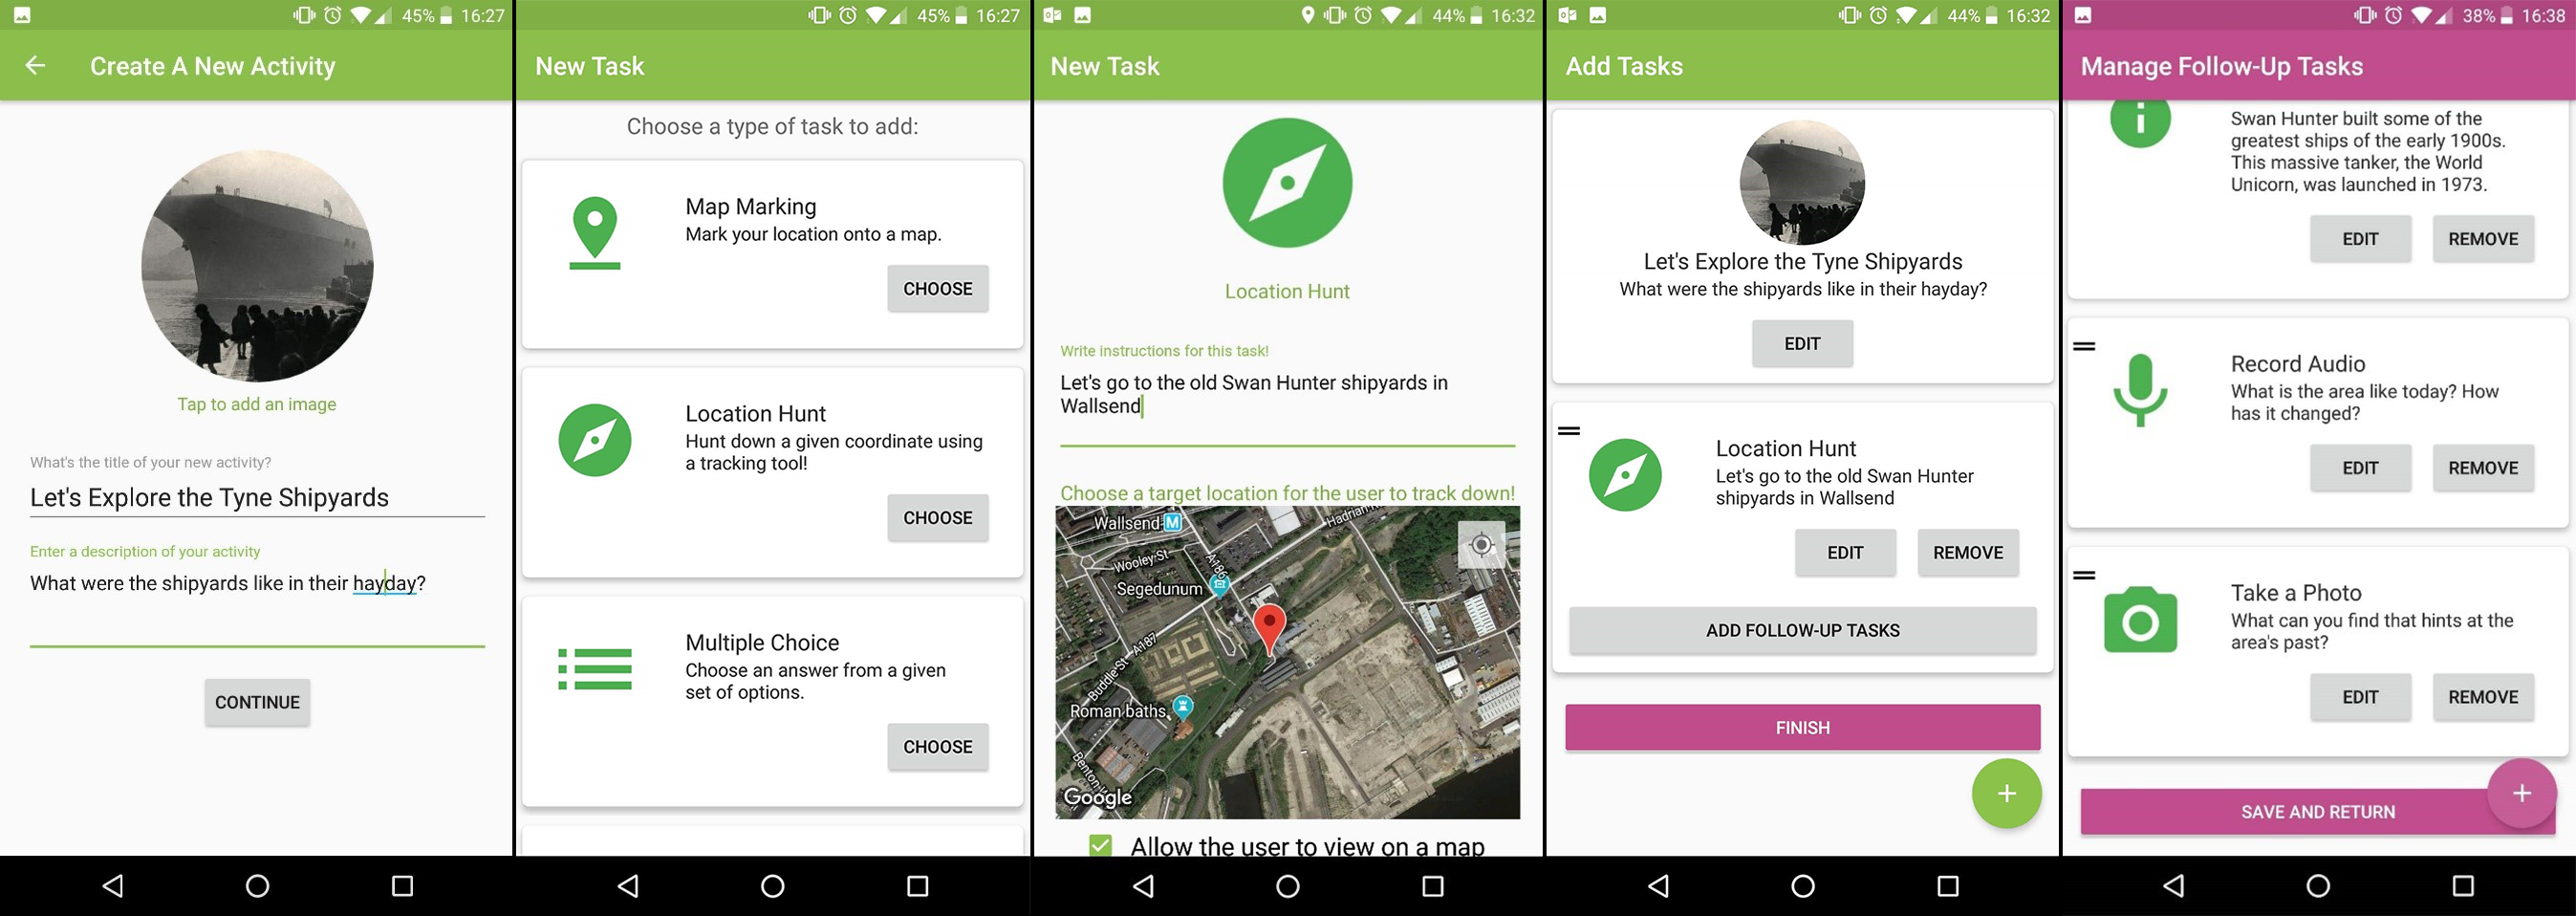
\includegraphics[width=2.1\columnwidth]{figures/activityCreation}
  \caption{Creating an OurPlace activity (left to right): a) Choosing the activity's title, description and image; b) Choosing a Task Type to add; c) Adding a \textit{Location Hunt} Task, with description and target coordinates; d) The new Task in the Activity; e) Adding Follow-Up Tasks to the \textit{Location Hunt}  }~\label{fig:ActivityCreation}
\end{figure*}

Activities are created within the app itself. After supplying a title, description and an optional image (Figure~\ref{fig:ActivityCreation}.a), the designer creates the Tasks that make up the Activity (Figure~\ref{fig:ActivityCreation}.b). Each Task Type requires at least a written instruction for the learner (e.g. A \textit{Location Hunt} might say \textit{`Can you find Carter's Well?'}), but some of them require some additional customization (e.g. supplying geographic coordinates by tapping on a Google Maps view) (Figure~\ref{fig:ActivityCreation}.c). No additional equipment or software is required to create activities (other than \textit{Scan the QR Code}, which requires creators to print the generated QR code from the OurPlace website). Uploaded activities can be edited for testing, feedback and iteration--allowing for the `essential elements' of reflection, critique and revision of a final public product \cite{Larmer2015}. 

\subsection{Overview of the OurPlace Curriculum}

From previously identified issues encountered by past researchers and practitioners when implementing project-based learning projects in schools \cite{Blumenfeld1991, Krajcik2006, InnovationUnit2016, TheEducationEndowmentFoundation2016}, we knew that any programme of activities would have to be able to adapt to variations in teachers' time and levels of mobile hardware access. In response, we designed an adaptable six-stage curriculum, which could span from dozens of hours of teaching time to only a handful (through omission of stages). This curriculum asks students (either individually or in groups) to create an OurPlace Activity as a final public entity, following a series of PBL engagements in response to their teacher's chosen topic. The stages are described below. While the curriculum was designed with the OurPlace application in mind, we believe it could be adapted for other learning technologies.

\subsubsection{Introducing the Medium}
This first stage involves the students becoming familiar with the OurPlace application: its feature set, the structure of an Activity and some examples of how the different Task Types can be implemented. This would ideally be performed with an example Activity, created to demonstrate all of the different Task Types available to the students. Doing this on the school grounds allows students to explore the application in a safe outdoor environment, and doesn't require the overhead of additional teaching assistants. This stage allows students to bear the capabilities of the technology in mind to help them formulate ideas during the following stages.

\subsubsection{Researching the Domain}
As with most other forms of PBL, a significant amount of time is allotted to students investigating the given problem domain. This is likely to be assisted in some way by technology, however other options exist such as fieldwork (e.g. site visits, performing interviews) and offline research (e.g. in libraries). A degree of autonomy should be granted to the students, however some guidance may be required.

\subsubsection{Prototyping}
In this stage, students create a low fidelity, pen and paper prototype of their Activity using their research as content. For this series of studies we created a `jigsaw' exercise, where students can design and play with different configurations of their OurPlace Activities without having to simultaneously learn the app's authoring interface (Figure~\ref{fig:JigsawToApp}). It also means that the students can start designing their Activities without access to mobile hardware. The jigsaw's structure is directly analogous to that of an OurPlace Activity: a single piece is dedicated to the Activity's title, description and cover image (i.e. Figure~\ref{fig:ActivityCreation}.a), with the Activity's Tasks represented as separate pieces connecting to it and chaining together. Each Task's jigsaw piece has a slot for a Task Type, and the jigsaw's connectors allow for pieces to be connected in different directions (e.g. to indicate Follow-Up Tasks). Pieces were given a layer of sticky-back plastic and written on with dry-wipe pens, allowing  both the students to make amendments and the jigsaws to be reused. Once students are happy with their configuration, the prototypes are photographed for later reference.

\begin{figure}
\centering
  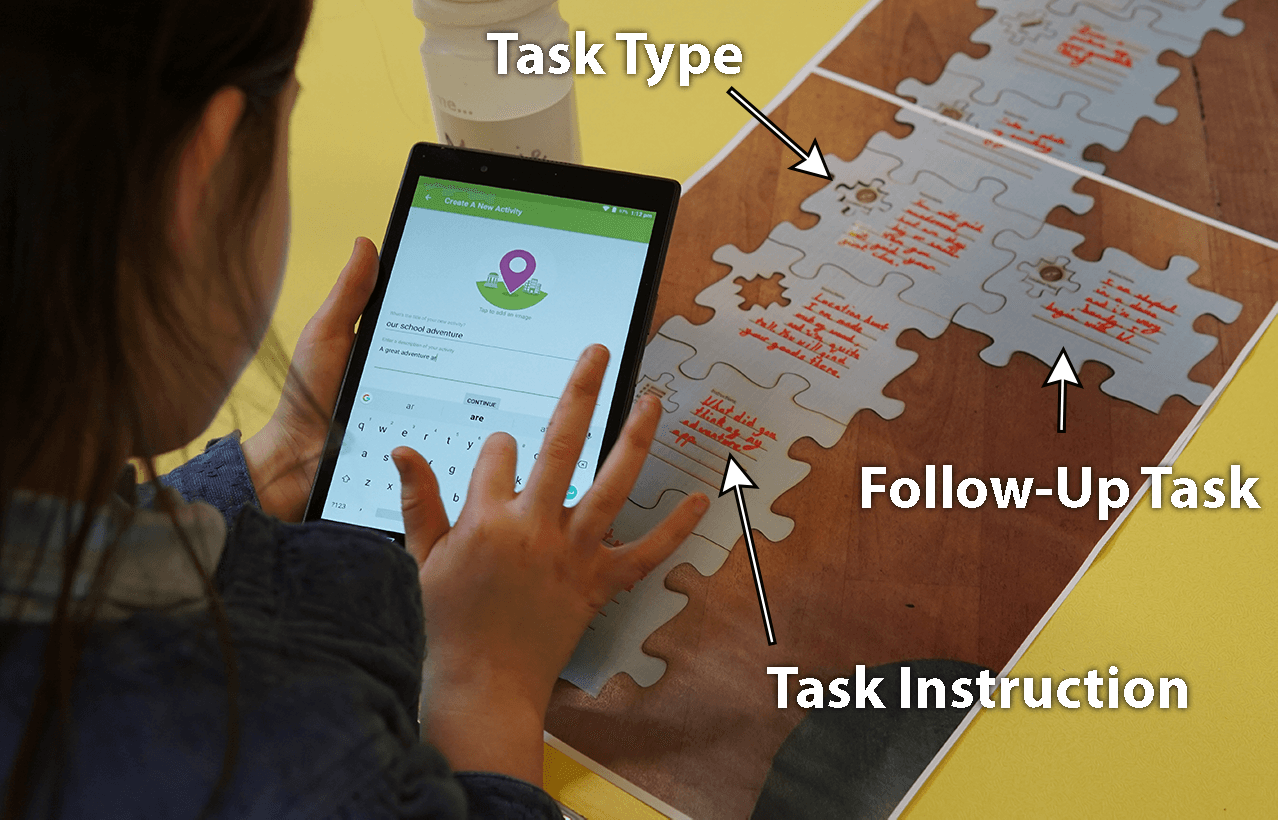
\includegraphics[width=1\columnwidth]{figures/jigsawToApp}
  \caption{A student uses a photograph of her jigsaw prototype as a reference for creating an OurPlace Activity.}~\label{fig:JigsawToApp}
\end{figure}

\subsubsection{Assembling \& Refining}

This stage involved the creation of the Activity within the OurPlace app itself, and requires some instruction from the educator/researcher as to how the app's creation process works. If the students created a prototype, this simply serves as a digitisation process. Once finished and uploaded, students may want to try their Activities (location allowing) and refine them in response to any issues they encounter.  

\subsubsection{Sharing with Classmates in the Wild}

With the final versions uploaded, students exchange Activities with each other and run them in the authentic learning environment. Ideally, this would also include an element of peer feedback afterwards.

\subsubsection{Sharing Externally in the Wild}

Students' Activities are framed as literal public entities, accessible within the authentic learning context for communities outside of the school.

\section{Studies}

We needed to assess how well this curriculum would work when applied within a real school context and how it could be configured to adapt to a given school's time and resource limitations. In this section we discuss studies held with three different formal education schools in the North East of England, as well as engagements held with a summer school of Travelling Showmen. Each has their own socio-economic and cultural backgrounds alongside a unique locality.

\subsection{Research Methods \& Data Collection}

All student interactions with the OurPlace application took place through Android tablets provided by the researchers, with the tablets' Internet connectivity provided by the researchers' wireless router and SIM card. The first author was present whenever the app was in use (unless noted), providing technical support as necessary and taking field notes and audio recordings. No identifiable information on the student participants was collected with the exception of photographs, which were only taken with prior parental consent. Any names given below are pseudonyms. Semi-structured interviews were held with the teachers after the engagements, with a mixture of oral and written feedback given by students. A thematic approach to coding was performed across all of this data, with codes being qualitatively analysed by the authors before grouped into final themes.

\subsection{Configuration 1: Extreme Time-Limitations (IR-A-\--)}
The first group we engaged with was a Year 8 history class (age 12-13, N=32) in a secondary school (School 1) based in a moderately affluent village. We approached the school's leadership about the possibility of them using the app: the school's headteacher agreed and assigned the class's history teacher (Teacher 1) to the study. School 1 appeared to have a very `traditional' teaching environment--as with many other secondary school teachers in the UK, Teacher 1 was under pressure to prepare the students for frequent formal assessments, and so was reluctant to dedicate much teaching time to the project. When we were organising the study, he noted: `\textit{Workload and time would be the main issues--the commitment it would take up in lesson time. It would be difficult to slot something additional like this in around key assessment work, and also keeping it relevant to the curriculum we are following}'. As a result, the project was given a very short amount of classroom time--only two hour-long sessions, with further work to be done by students outside of school. Observations of two of Teacher 1's other lessons suggested that he preferred an `authority' or lecture style of teaching: lessons were teacher-centred, with students expected to take notes on content that was delivered to them and answer occasional questions raised by the teacher. Teacher 1 appeared ambivalent towards PBL approaches, and when queried on his opinion of them simply noted `\textit{It's not the way we do things here}'.

Teacher 1 already possessed a paper-based history trail of the local village, designed for use by new, younger students joining the school. For the study, Teacher 1 tasked his class to use OurPlace to create a digital trail, featuring historical elements of their choosing. Prior to our first session with the students, he provided them with a comprehensive and lengthy PDF document, which detailed most--if not all--of the historical buildings in the village, serving a starting point for researching content. He also provided the students with the existing trail and a PowerPoint presentation containing information pulled and summarised from the PDF. As a result, prior to the first session, Teacher 1 expected that the students should be fairly well prepared in terms of trail content: `\textit{The students should already have ideas of what they want to do, but are waiting to see what the software will do. The issue is what the software can do and whether it can easily tied in with the plans they have made already.}'  As such, the \textit{Researching the Domain} stage was present, albeit earlier in the process than we had anticipated. 

Teacher 1 was also concerned about the students' work being able to work outside of a mobile learning context, hoping to also have `analogue' versions of the students' trails: `\textit{Ideally, what is done needs to be able to be adapted to be used again. The bespoke software side of it does worry me a bit in this regard. Could a finished product be adapted to be used at another time even if no iPads were available--maybe some of the ideas usable in a non-digital way?}'. To this end, he encouraged students to try and design their digital trails such that they would be adaptable to a pen and paper format.

Teacher 1 decided to make the majority of the Activity creation process a homework task, with students using their own smart devices outside of school. This was mainly in response to the extremely limited amount of classroom teaching time that could be dedicated to the project: because we also wanted to go through the students' final Activities with them, that only left a single hour-long session to work with the students in class. In order to prepare the students for this independent work, our first hour-long session was spent \textit{Introducing the Medium}. This involved the students completing an example OurPlace Activity on the school grounds, demonstrating all of the Task Types and several instances of Follow-Up Tasks. Upon return to the classroom, the rest of the session (around 20 minutes) was spent introducing the students to the Activity creation tools in the app. By the end of the hour, all students reported that they understood the app, what it could do and how to make their own Activity.

We returned to the school three weeks later for the second session, in which the first author and Teacher 1 sat with the students and went through their Activities with them. While most of the students had produced an Activity, they tended to be quite short (averaging X Tasks per Activity) and shallow: most of the Activities served more as explorations of the different interactions possible with the app than a meaningful engagement with the subject matter. For example, one student's Activity asked the learner to simply find and photograph an `area of interest', putting greater focus on the technology than the learning content. Despite this, many of the students had clearly engaged strongly with the process and had taken ownership over their Activities: for example, one student's trail featured characters she had created for her YouTube channel. However, as a result of the focus on technology interactions, many students struggled in fulfilling the teacher's requirement of creating a paper-based version of their Activity. One pair of students had more success, claiming `\textit{I think we've found it easier than other groups because we focused more on the content than using all of the different interactions. So a lot of the content can be the same, it's just changing how to interact with it}'.

When giving feedback to the class, Teacher 1 pointed out that even where their Activities might contain some meaningful content, they aren't necessarily good for learning from: `\textit{What needs some further thought is what you're actually asking them to do in terms of the content. What are they doing in order to get that information? They can't pluck things out of thin air if they have no idea. Feed them some information, then wherever they are at they can work out the rest.}' He then offered some ideas of how the features of the technology could be used as a teaching tool: `\textit{Or send them specifically to somewhere where they can work out the answer to something. Use of old images in this technology I think might work. You know, send them to a place with an old photograph. Get them to do some comparisons, get them to think about why things have changed}'.

Teacher 1 had also noticed the students' focus on interactions with the technology over engaging more deeply with the historical content. In the follow-up interview, he noted: `\textit{I don't know about you but the thing I was coming across again and again was the lack of challenge, the lack of depth, and the kind of things they were asking was really just playing with the technology rather than [engaging with the history]}'. This surprised him, as he had been expecting any issues encountered to have resulted from the introduction of new technology, rather than the students' research--especially as they had been given the resources so early on: `\textit{I think it's more of a success for the technology, the medium, than the actual content. [...] Maybe not what I expected, actually--in some ways maybe the opposite}'. He argued that without the deeper integration of research and knowledge into the Activities, they are of little value: `\textit{It needs to be worth doing: there's no point in having all of the bells and whistles if there's no substance}'. He noted that this could have been improved through a reconfiguration of the engagements, suggesting that more structured, scaffolded activities could have guided the students to produce more successful projects: `\textit{It's worth cogitating about what parameters you probably need to introduce, to guide them towards deeper thinking. I know that if that had been more free-form and open-ended, that would have been rather worse}.' He suggested that when applying content knowledge to Activities, a balance needed to be struck between a more guided, restrictive approach and supporting students' creativity and autonomy: `\textit{If they were highly creative and lost their focus, then they'd be miles [off]. If they were less creative, but focused on the nature of the content, they'd probably find it easier to transpose. What we want is something in-between}'.

\subsection{Configuration 2: Without Sharing Externally (IRPAC-)}
We worked with two different schools over an extended period of time (10-12 hours of sessions per school, spread over several weeks) to deliver a more fully-implemented version of the curriculum. This was partly supported by the fact that we were working with Year 4 (age 8-9) classes in both schools--as less focus is placed on preparing for examinations at these early ages, we've found (anecdotally, through previous research engagements) that pre-secondary school teachers are more willing to engage with experiential and exploratory forms of learning, rather than simply `teaching to the test'. As such, both schools welcomed the implementation of a longer project spread over several sessions.

\subsubsection{Engagements with School 2}
The first of these schools (School 2) was based in a tiny rural village, and--due to the small population--we worked with the entirety of the Year 4 group, who were the oldest children in the school (age 8-9, N=7). Because each the school's population is so small, the school's classes are actually made up of several year groups--meaning that Year 4 and Year 3 share the same classroom. The class teacher (Teacher 2) had approached us about using the OurPlace app as a way to augment orientation and map-reading with new technologies in lessons. With this generous scope and large amounts of time available, we decided that the students would do two projects: one to learn the mechanics of making Activities in the app, and another which focused on local heritage in the village. 

For the first project, we tasked the Year 4 students with creating OurPlace Activities for their younger classmates to complete, with the only stipulation being that the Activities should be based around the school grounds. A Teaching Assistant was present throughout this first project, to help the lead researcher with any children who struggled. As with School 1, in the first two-hour session we \textit{Introduced the Medium} through an example Activity which demonstrated the app's capabilities. We then moved straight to the \textit{Prototyping} phase, as these first projects didn't require any research. While the students initially struggled conceptually with the jigsaws due to their abstract nature, after a few minutes they understood the links between the puzzle pieces and the structure of the app. We soon found that while students were generally favouring the Task Types which they found most interesting during the demo Activity--namely \textit{Take a Photo, Location Hunt} and \textit{Record Audio}--their Activities made use of most of the different Task Types available. We believe that this may have been encouraged by the jigsaw packs having a limited number of each Task Type piece, meaning that students were unable to make an Activity with many of the same Task Type (however, some students overcame this by simply not placing a Task Type piece if the right one wasn't available--see Figure~\ref{fig:JigsawToApp} as an example). The largest hurdle was around students' ideation of what the Activities should be about--with such a broad scope and without a subject focus, they struggled to think of different themes. They all settled on some form of `adventure', where each Task was a puzzle or riddle to solve in order to find locations within the school. The students' jigsaws were photographed at the end of the session.

In the second two-hour session, during which the students \textit{Assembled} their OurPlace Activities, the photos were given to the students as references   (Figure~\ref{fig:JigsawToApp}). One of the students particularly struggled with typing with the on-screen keyboard, which Teacher 2 attributed to due to lower literacy skills. However, the others were happy working independently, and reported that their jigsaws made learning the creation process `\textit{much easier}'. The students had fun exploring what they could do with the app's functionality: for example, one student's final \textit{Listen to Audio} Task `rewarded' the user for completing his Activity with a recording of him singing \textit{Celebration} by Kool \& the Gang. The second session concluded with the students testing out their Activities and making a few refinements (mostly involving spelling errors and re-ordering Tasks). 

\begin{figure}
\centering
  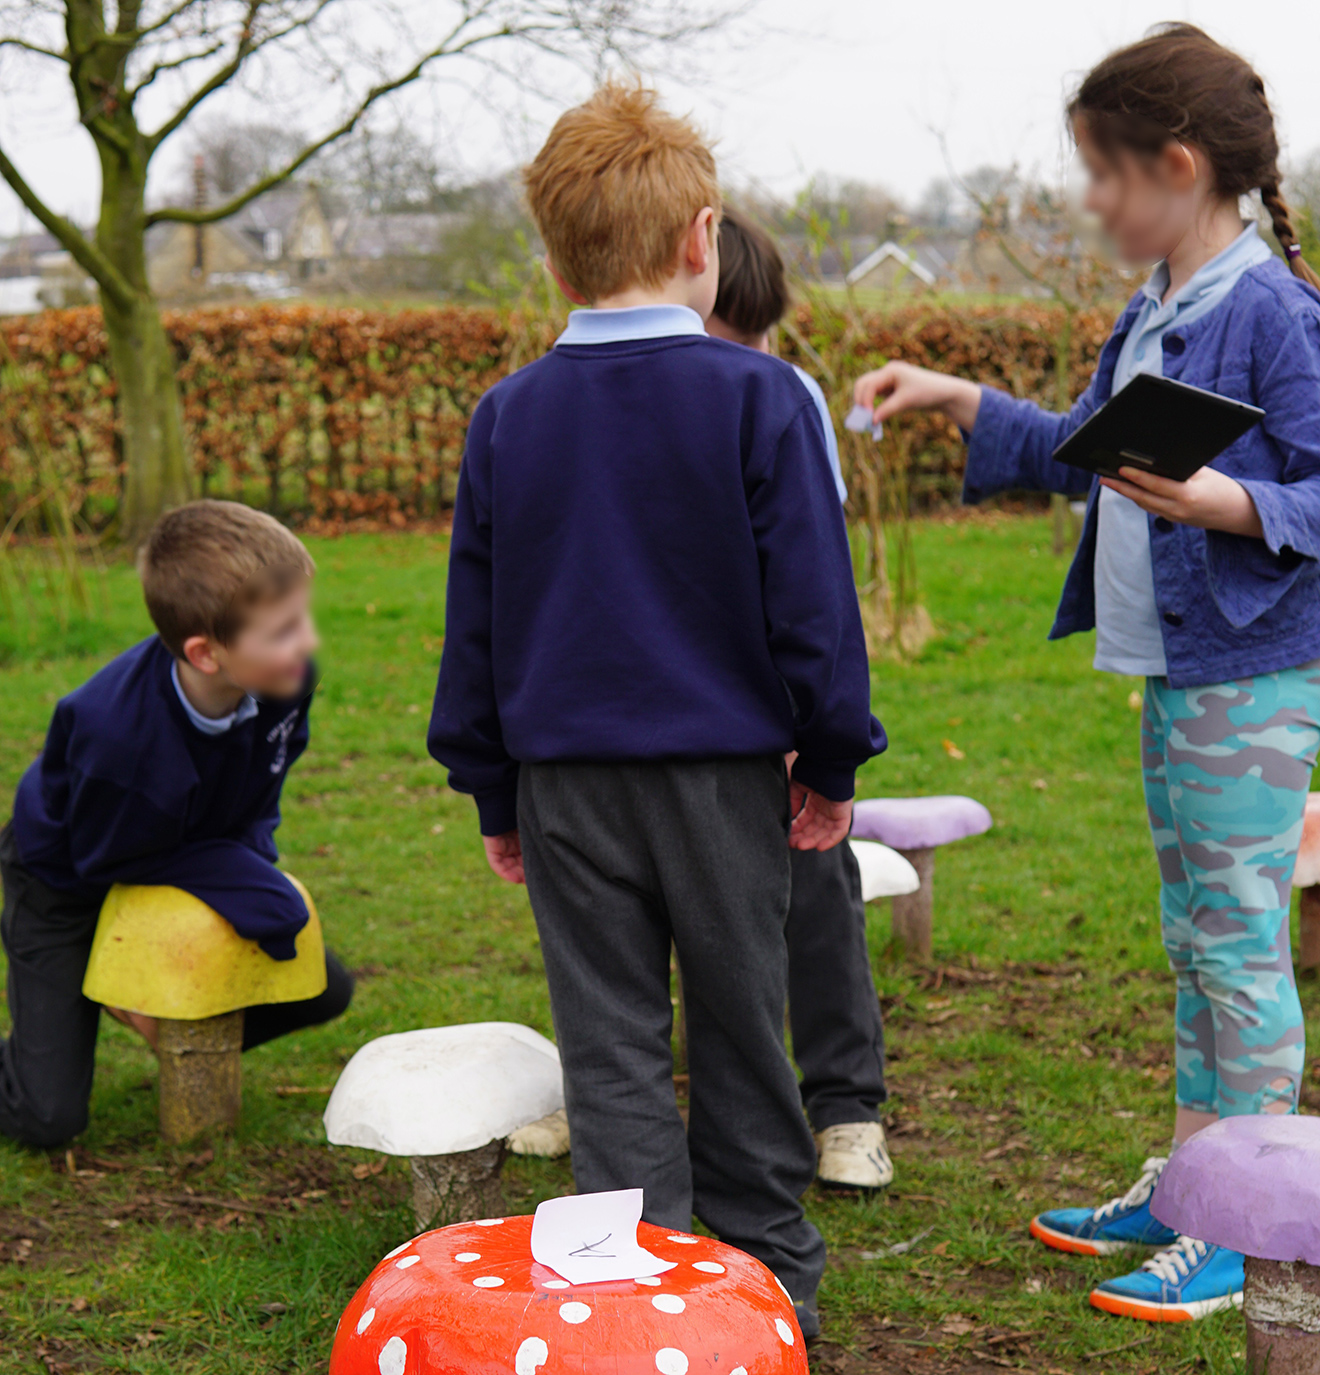
\includegraphics[width=0.8\columnwidth]{figures/mushrooms}
  \caption{A Year 4 student reveals a clue to her Activity's next puzzle. }~\label{fig:Mushrooms}
\end{figure}

The final two-hour session of the project was spent by the students \textit{sharing with their peers}. Teacher 2 briefed the younger students, giving the Year 4s positions of seniority and highlighting their efforts: `\textit{You really need to listen to what [Year 4] have to say, because they have designed this themselves. They are your teacher, OK? Please listen, because they've worked really hard, and they're really excited about you having a go.}' The Year 4s accompanied rotations of small groups of younger students as they completed their Activities around the school, with groups being swapped to allow all students to try each Activity. The Year 4s were given the responsibility of showing the younger students how the app worked, and assisting them if they got stuck (Figure~\ref{fig:Mushrooms}). The younger students were very enthusiastic, and were keen on making sure they completed each of the Year 4s' Activities. At the end of the session the Year 4s hosted a school assembly, in which they showed the other children their jigsaws and shared what they most enjoyed (`\textit{I enjoyed being the teacher'; `Being outside'; `I enjoyed making the Activity itself}') and the younger children gave them feedback (\textit{`Our favourite was [Susan's], because we got to find lots of things'; `I really liked the beeping one, the Location Hunt'}). The school's headteacher praised the Year 4s' independent work as showing maturity: `\textit{We can trust you to do something away from the class teacher and still do something really good. I think you really are stepping up to be Year 4s, it's wonderful to see. [...] If you're very grown up, you get to do very grown up things. So let's give year 4 a clap}'. Teacher 2 also praised their leadership (`\textit{I would like to also point out how good they were as teachers, as well. They really came into their own. I was very proud of them.}') and noted that the OurPlace app supported a varied output: `\textit{They were very different as well weren't they? The ideas. Even though you all started off with the same tools'}. Finally, the headteacher noted that the Teaching Assistant had also been strongly engaged with the process: `\textit{Gabrielle said she was going to stay extra time, because she wanted to see how it was going to finish up. She worked overtime so she could see how [Year 4 were] getting on. So she was really interested as well}'.

Following the success of the first project, Teacher 2 was excited to start the second one. Prior to the lead researcher's arrival at the school to begin the second project, she had preemptively collected a number of historical resources relating to the village, including newspaper articles, photographs and a book detailing the village's buildings. As Teacher 2 claimed to not have much prior local historical knowledge, this also served as her introduction to the village's heritage. She proceeded to make a shortlist of the more interesting buildings (such as an old blacksmith, a pub and a post office), shared these with the Year 4 students, and then took them on a short walking trip around the village so that all of the children had first-hand experience with them. Each child chose a different location to base an Activity on.

As the group was already familiar with the OurPlace app, we skipped the \textit{Introducing the Medium} stage. Furthermore, when we asked the students if they would find it helpful to plan their Activities out using the jigsaws, they said no: they'd rather jump straight into making them using OurPlace, as they were already comfortable creating and editing using the app's tools. The Activities were produced over three hours between two sessions, with the remainder of the second session consisting of the students sharing their Activities with each other and the younger students. The children were split into three groups, with each group accompanied by an adult and sharing tablets one-between-two. The groups completed each of the Activities around the village before returning back to the school. While the Activities created by the students were simplistic (Figure~\ref{fig:Mushrooms}), Teacher 2 was satisfied with them, as they served as a medium through which `\textit{they were able to engage with the local history in a way which they enjoyed, and they've taken pride in sharing their work with the Year 3s}'. Following the trip, several of the younger students asked if they'd be able to make their own Activities the following year.

\begin{figure}
\centering
  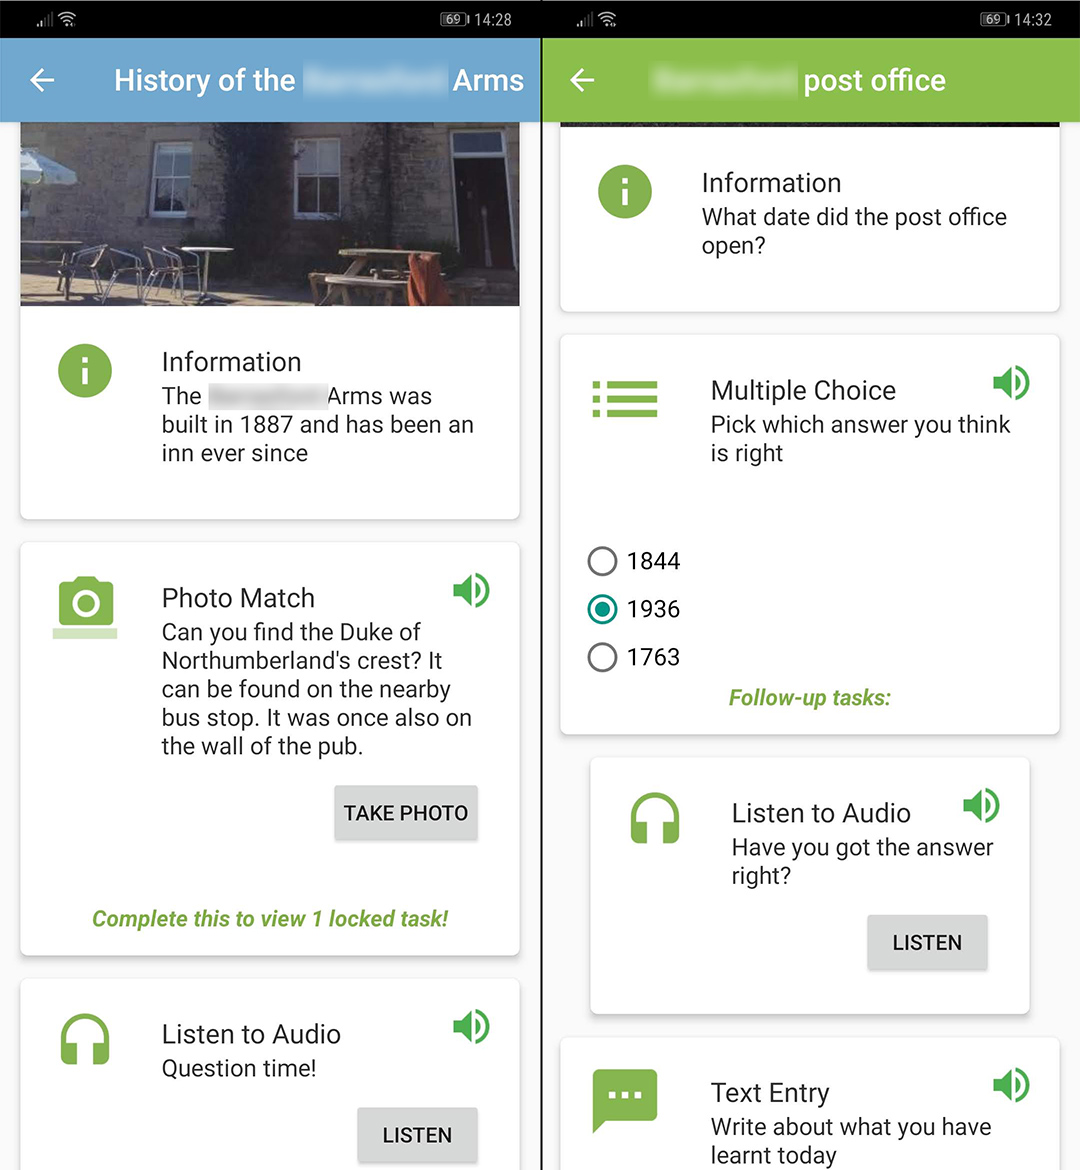
\includegraphics[width=0.9\columnwidth]{figures/createdActivities}
  \caption{Activities created by Year 4 students about their village's buildings of interest. }~\label{fig:CreatedActivities}
\end{figure}

\subsubsection{Engagements with School 3}
We approached another Year 4 teacher (Teacher 3) at an inner-city school (School 3), after her class had shown an interest in local history by successfully campaigning for the installation of a commemorative plaque. The plaque celebrated a notable slavery abolitionist who had lived near their school, and was particularly notable due to School 3 being based in an ethnically diverse, disadvantaged area and serving a large number of families of Nigerian descent. Teacher 3 was enthusiastic about the concept of producing Activities relating the the area's numerous other plaques. We worked with the majority of the school's Year 4 (age 8-9, N=21, led by Teacher 3) and Year 6 (age 10-11, N=32, led by Teacher 4) students, who worked together on the project in mixed groups.

As with School 1 and School 2, the students used a demonstration Activity as an introduction to the app. Following this, Teacher 3 explained that each group was to choose and research one of the historical figures commemorated by the plaques in the area, and produce an Activity related to them. Over the following week, the teachers dedicated a couple of hours of class time to researching the plaques and going to visit them. As a result, by the second engagement each group had prepared several pages of notes relating to their chosen plaque, and they were ready to start constructing their Activities.

While the School 2 students created their prototypes immediately after completing the demonstration Activity, the School 3 children started their jigsaws a week afterwards. As such, they were less familiar with the structure of the OurPlace app, and found it helpful to have a tablet for reference while constructing their prototypes. The students frequently referred to their notes while writing their Tasks, and some groups even designated roles relating to writing different Tasks and designing the Activity's overall structure. The completed jigsaws were photographed and used as references for creating the Activities in a third session later that week. Part of this third session was also spent visiting the plaques with the students, so that they could test and refine their Activities and take photographs to include in them. The final session of the project involved the students going out for a second time, and completing each other's Activities. The students' final output of the project was mixed, with some Activities lacking content. This was attributed to numerous causes, including technical issues (two groups' progress was deleted due to a bug in the application), a lack of available information for the chosen plaque's subject, and how several students exhibited behavioural issues.

When asked what their favourite part of the project was after the final session, several of the students mentioned that they particularly enjoyed sharing and seeing each other's Activities: `\textit{[I most enjoyed] today, getting to go around and swap with other people and getting to find out about theirs}.' They also noted that they felt that swapping Activities was an important part of the process, as it could also share different ways in which the Task Types could be used. Furthermore, one Year 6 student recognised that the OurPlace app could be used to share knowledge about and the value of place with visitors and other communities: `\textit{I think that if we made stuff for another school that made them learn, it would be really good because you could make it about your school.}' Teacher 4 expanded on this concept: `\textit{That's a very different school experience to what you have here, so that would be an interesting thing to do, wouldn't it? To swap it and see what their daily life is like and what yours is like.}' 

During a follow-up interview with Teacher 3 she noted that she particularly liked the tactile and visual nature of the jigsaw prototyping activity, and how students engaged with it: `\textit{I definitely liked the jigsaws. If you're doing it on a piece of paper it's very boring, isn't it? So to get them to fit in, and to get them to understand that the order can matter... I think that's a very good, visual way of showing the children: they like jigsaws and it's fun. That really worked.}' Unlike the children in School 2, she also saw value in doing the prototyping for making further Activities: `\textit{I would use the jigsaws every time. Because it's a different activity. Sort of like a brainstorm.}' In this regard, Teacher 3 recognised the jigsaws as Activity prototypes, rather than simply a way of easing the students into the application's structure. Following the study, she requested the jigsaw's file so that she could print copies and use it with students to prepare future OurPlace Activities. Teacher 3 also saw a potential value in exchanging with separate groups of students, noting that time pressures can become a limiting factor: `\textit{I think that would have been better: if we'd done it, and then taken a different group of children out to use it. So you do it with one class, and when they finish, take the other class with them to show it. And then they can evaluate by watching the other child. But it's just time pressure, isn't it?}'

Teacher 3 was also highly favourable of teaching in authentic contexts and using local civic spaces as learning resources, as the children already had a grounding: `\textit{It was all about taking a context specific approach, and that's what I'm really into. These children know about their local area, and that helped us scaffold the Activities.}' However, she was also aware that many of the children were not aware about the area's history, and the historical figures could act as inspirational role models: `\textit{This is where the children live, so it's really important that they understand the history of it. Some really great people who're like them have lived in this area}'. Furthermore, engaging in these shared environments brought the children in contact with local community stakeholders: `\textit{They got to meet people when they went out and about. They met Jeff from the bowling club, and they met the guy who's raising money for the Frederick Douglas sculpture in the middle of the park}'. She also recounted that the students had even shared some of their newly acquired knowledge with community members while completing the Activities: `\textit{When we went to the Joshua Alder house there were two ladies. They'd seen the house on TV, they were coming to have a look at the plaque, and they were asking about the house next to it. We knew was a synagogue because we'd done the research first for making the Activities. Already sharing knowledge!}' Teacher 3 also argued that using the OurPlace app in a PBL approach helped her leverage these civic resources in her lessons, as the creation of public entities acted as a motivating factor: `\textit{We'd done a lot of research on Frederick Douglas, but it was how we were going to bring those other people into our lesson. I think that OurPlace really helped: it gave us a focus to do the history through the app, rather than just go and collect the information and then--"what do we do with it?"}' 

\subsection{Configuration 3: Sans Introducing the Medium (-RPA-E)}
Through discussions with Teacher 3, we discovered that she spends a period of the Summer school term leading a summer school for children of families who run the local annual funfair. Following our engagements with School 3, she invited us to run a short engagement with a group of children (age 6-9, N=16) attending her summer school. These were the children of Travelling Showmen and Showomen, members of the Showmen's Guild: a trade association made up of traditionally insular cultural groups of families, who travel around the UK to run funfairs and circuses. While the children of these families (Showchildren) are registered with traditional schools, the families travel so frequently (one family claimed to work 40 events a year) that their schools send out packs of educational materials for the children to work on remotely. Teacher 3 derided these worksheet-based packs as uninteresting: `\textit{[The school packs] are super boring and often rubbish. Some schools are alright, but it's still working from a piece of paper.}' Inspired by Teacher 4's suggestion that OurPlace could be used as a medium through which daily life experiences could be shared, Teacher 3 suggested that we do a short project at the summer school: `\textit{Their lives are so different, it would actually be a nice tool to share with other children what it's like to be a Showman. [...] The children would love to do something, because as I say their work packs are super dull.}' We decided to arrange a trip for the Year 4 class from School 3 to visit the fair, where the Showchildren would introduce them to their ways of life and use the OurPlace app as a form of mediating tool or for supplementary material.

As the summer school only ran for two weeks, we had limited time with which the Showchildren could create their Activities. We only had one three-hour session in the summer school in which to introduce the children to the app and have them create Activities, so we decided to try another configuration: skip `\textit{Introducing the Medium}', and rely on verbal instruction during the prototyping stage as an introduction to the app's functionality. The jigsaw activity proved to be intuitive enough to make sense to the children without them first needing to use the application, as very few of the children struggled. Most of the Showchildren gravitated towards making Activities which focused on their families' rides and stalls within the fair, with a few children instead focusing on the largest attractions which interested them personally. The children also generally favoured camera-based and drawing Task Types, using far fewer \textit{Location Hunts} than the other groups had. This was likely due to the fact that they could intuit what \textit{Take a Photo} would involve, whereas \textit{Location Hunt} benefits from further explanation and demonstration. Transitioning from the jigsaw prototypes to building the Activities in OurPlace went as smoothly as it did in the previous engagements, suggesting that the jigsaw serves as an intuitive metaphor for the application. Due to time limitations, the Showchildren were unfortunately unable to test and refine their Activities.

To prepare the Year 4 children for the trip, we then ran a session in School 3 to introduce them to the concept of Travelling Showmen. Several of them already had a base knowledge of the community, thanks to Teacher 3 talking about her experiences running the summer school. For example, they already knew that the Showchildren `\textit{help their parents with the rides}' and `\textit{[deal with] money, they're good at maths, giving people change}'. The Year 4 class's discussions largely centred on the concept of the Showchildren working in the fair, an idea which appeal to them: one child noted he wanted `\textit{to get money to support my family}'. However, there was a concern that as children, they wouldn't be treated as equals by adults: `\textit{you might not get paid as much, because people could want to only go to adults and think that children are not responsible yet}'. Furthermore, the children found the idea of inherited careers generally unappealing (most Showmen families have a lineage of several generations within their occupational community). Many children noted a desire to diverge from their parents' careers, saying `\textit{I don't want to do my parents' job}', and `\textit{it's natural to want to do something different, [...] if you just carried on a tradition you might not really like it.}'

To encourage fruitful conversation between the two groups of children, we also asked Year 4 to prepare some questions to ask the Showchildren. Many of the questions prepared by the class revolved around the Showchildren's independence and influence in the community (e.g. `\textit{Have you ever designed a ride?}', `\textit{What rides have you built?}'), their work-life balance (`\textit{Would you like shorter or longer shifts?}', \textit{`What do you do when you've finished work?'}) and even the Showchildren's earnings (`\textit{How much money do you earn?}', `\textit{What's your net worth?}'). The class also believed that the Showchildren's contributions would make them privy to knowledge about their family's financial earnings. Comparatively few of the Year 4s' questions focused on the social and lifestyle aspects of the Travelling Showmen community (e.g. `\textit{Do you have any relatives who are in a different part of the world?}').

The trip occurred the following week, with Year 4 travelling by coach to the fair. An education specialist from the Showmen's Guild gave a short talk to the children regarding Showman ways of life, and her experiences growing up within the community. Following this, the Showchildren and Year 4s were put into small mixed groups of 4-5. Each group were given two tablets with the Showchildren's OurPlace Activities pre-downloaded, and the Showchildren were instructed to guide the visitors around the fair. As they were navigating a working environment with heavy machinery, large vehicles and a limited line-of-sight, the groups largely had to stay together so that they could be observed by the teachers present. Unfortunately this limited the children's ability to explore the fair and visit all of the locations present in the prepared Activities.

As well as follow the Showchildren's OurPlace Activities as intended, the Year 4s also used them to structure their data collection, using the app to catalogue photos of the different rides and using the \textit{Record Audio} and \textit{Record Video} Tasks to capture the Showchildren's responses to their prepared questions. While some of these questions were still relating to the Showchildren receiving money (`\textit{Do you get any of the money that your parents get?}'), most of them had shifted to questions about the lived experience of being a Showchild (`\textit{How long have you been in [anonymised] for?}', `\textit{In a year how many places do you think you travel to?}', `\textit{Do you get to make many friends outside of the fair?}'). The Showchildren also responded with a couple of questions of their own, querying the Year 4s' experiences with the fun fair.

One of the Showchildren was particularly interested in the functionality of the OurPlace app and creating more involved Activities. He was particularly excited for the Year 4 students to complete his \textit{Scan the QR Code} Task, which asked them to find his parents' ride: `\textit{We're near my ride! Can you go scan a QR code that's on the gallopers, just over there?}' However, when it was scanned he was disappointed to find that it didn't unlock anything, as there weren't any Follow-Up Tasks set. When this was explained, he clearly didn't know what Follow-Up Tasks were: `\textit{What did you mean by follow-up? How do you put something in it?}' While disappointed, he expressed interest in downloading the app himself and making more detailed Activities in his own time.

\section{Discussion}
These studies have shown us that the different ways in which mobile learning engagements can be configured can have significant impact upon how the technology is seen and utilised by its users. They also highlighted how by supporting creativity as a teaching objective, these technologies can offer children outlets for independence and personal flair within their studies, and new avenues for teachers to leverage local places as learning resources.

\subsection{Configuration and Compromise}
In these studies it was necessary to adapt our created OurPlace curriculum in response to each teaching context. A common element across most of these contexts was time limitations: for example, Teacher 1 was severely limited in how much time could be dedicated to the project due to obligations to follow a strict curriculum, while the Showmen's summer school was only running as long as the funfair was in town. It was only when working with the younger classes in School 2 and School 3 that more time could be afforded. This was certainly not ideal for PBL-style engagements, which should engage students over the course of an extended period of time \cite{Blumenfeld1991}. Nevertheless, we argue that teaching contexts are rarely ideal, and so approaches to working within them should be adaptable and open to compromise. For this reason, we wanted to see how `compromised' configurations of the curriculum performed when implemented in real classrooms. 

As Teacher 1 seemed confident that his students had ample resources for the content and was more concerned about their lack of familiarity with the OurPlace app, we decided that we would focus our time on \textit{Introducing the Medium} and use the \textbf{IR-A-\--} configuration. This skipped the \textit{Prototyping} and both \textit{Sharing} stages, which we believe contributed towards the lack of engagement with the domain and put the students' main focus on the technology itself. Before taking the project away as homework, the last classroom engagement the students had with the project was the demonstration of the technology, meaning it was likely to take centre-stage in their minds. Our observations at School 2 and School 3 suggest that had it been included, the prototyping jigsaw Activity may have brought the students' focus back to the domain's content. Furthermore, the lack of emphasis on sharing the created Activities with either their peers or outside communities may have also made them seem less important to the students, as them not being socially shared reduced their value as constructionist `public entities' \cite{PapertSeymourandHarel1991a}. Teacher 1's skepticism towards and lack of experience with the PBL model may have been another compromising factor, as it has been argued that successfully putting it into practice requires both teachers and schools to fully commit to substantial changes in classroom structures and approaches \cite{InnovationUnit2016}.

In response to these findings, our other time-limited engagement with the Showmen's summer school used a different configuration, in which we skipped the \textit{Introducing the Medium} and instead focused on the \textit{Prototyping} stage (\textbf{-RPA-E}). While the jigsaws seemed to provide a somewhat serviceable introduction to the app due to the closeness of its metaphor, the full capabilities of the technology had evidently not been made clear to the Showchildren. In the case of the Showchild with the QR code, this resulted in a degree of frustration and disappointment that his Activity wasn't as fully featured as it could have been. It's unsurprising that more advanced functionality, such as Follow-Up Tasks, would be unclear to children without first demonstrating them in an example Activity.

The studies also highlighted the value of the latter stages of the curriculum, in which students share their creations with their classmates and/or the wider community. Students from School 2 and School 3 emphasized the exchanging of Activities as being a particular highlight of their experiences, with students keen to both see what their peers had produced and also show off their own creations. Teacher 3 noted that had time allowed, she would have extended this sharing stage further, in order to support peer feedback between classes and groups.

Each of these configurations held their own compromises, resulting in an interesting balancing act between three main elements: supporting the learners' understanding of the technology medium (omission led to not using the technology's full potential); supporting the meaningful application of content knowledge to that technology (omission led to shallow public entities which focused on the medium rather than the content); and enabling learners to exchange their creations, knowledge and feedback within authentic learning environments (omission reduced the value of the entity creation process). Each of these elements proved to be important, and compromising on any of them while still producing successful PBML engagements was difficult. However, successive projects can mitigate this issue, as stages can theoretically be omitted as the learners become more comfortable with the technology. This was shown in the second set of Activities made at School 2, where the students no longer needed to be introduced to the app, and even opted to skip the prototyping stage. However, even this was up to some degree of teaching interpretation, as Teacher 3 noted she would use the jigsaw prototypes each time her class made new Activities. 

\subsection{Harnessing Students' Desire for Independence}
In these studies, many of the students we engaged with had a great desire for autonomy, independence and to be respected as individuals. This was particularly reflected in the School 3 class's fascination with the Showchildren's contributions to their family businesses; their lamentation at their lack of perceived responsibility when compared to adults; and the class noting their desire to start working in order to financially contribute to their families. They also voiced a desire to walk their own path rather than simply emulate their parents: eschewing tradition and inherited jobs, instead favouring personal happiness and fulfillment. 

The PBML process appeared to capitalise on this quality, granting the students a greater amount of control and autonomy over their work and allowing them to approach creating their Activities with greater degrees of personal input. This could be seen in some of the personal touches put into their Activities, such as the Year 4's rendition of \textit{Celebration}, or the Year 8's usage of her YouTube characters. These flourishes--alongside the uniqueness of each Activity--suggest that OurPlace conforms to Noss and Hoyles' requirement that constructionist tools should be expressive enough to support exploration and ownership through construction \cite{Noss2017}. This also echoes previous research held with OurPlace's predecessor, ParkLearn, in which students' sense of ownership of their work (promoted by greater degrees of freedom and independence) was an important contributing factor towards their enthusiasm \cite{Richardson2018}. Furthermore, the students' investment in their projects supports previous research which argued that the greater autonomy afforded by PBL, as well as tapping into students' fluency with technology, can result in greater levels of student engagement \cite{Wurdinger2007, Bell2010}.

When sharing their Activities with their peers, the students were clearly proud of their creations and enjoyed taking a `teaching role': they took care to guide the other students through the Activities to avoid them getting stuck without being overbearing. The School 2 teachers rewarded the students' performance by playing to their desire for perceived maturity, noting their growing trust in the children to perform independently and recognising their seniority amongst the students. As this took place in a school assembly, this feedback also served as qualities for the younger students to aspire towards--some of the younger students later enquired about making their own Activities when they're older. This move to reposition the Year 4 students from a `consumer' role to one of mentorship--in which they have a degree of authorship over teaching materials--mirrors the study by Massey et al, in which they re-framed students from end-users to software developers and decision makers \cite{Massey2006}. In both cases, the learners were empowered through the creation of public entities to be able to take an active decision-making role in how technology could be used within their learning environment. The addition of the \textit{Sharing} stages took this a step further, granting the students the gratification of seeing others enjoy their creations.
 
We suggest that future mobile learning designs can harness student's desires for independence as a motivational force by granting them opportunities for autonomy and personal flourishes, as well as platforms through which to share these personal creations. Within these studies, this was achieved through a combination of technology and configuration: OurPlace elevated students from consumers to producers by granting them creative control, and the creation and sharing of public entities in the culmination of a PBML process bolstered their self-worth and empowered them through positions of mentorship. However, it's also worth noting this approach may not be conducive to success in all contexts, as teaching styles and cultures within different schools may be at odds with it or require re-balancing. For example, Teacher 1 was in favour of greater levels of scaffolding, and believed that further student autonomy and creativity would be detrimental. 

\subsection{Leveraging Local Heritage through PBML}
Project-based mobile learning offered new ways and motivations for the schools to engage with their area's local heritage, surfacing `new' educational resources which had previously gone underused. For example, Teacher 2 reported to previously know very little of the village's local history, and School 3 hadn't previously made use of the commemorative plaques as learning resources. Teacher 3 argued that using OurPlace to create the public entities gave lessons a focus and motivation needed in engaging teaching sessions, as simply collecting information would have felt aimless. She was also ardently in favour of the students learning more about their local context, as the historical figures within the area could serve as inspirational role models. Finally, in the Showmen study, a (compressed) PBML process also supported exposure to and greater understanding of another community's heritage. The students' preconceptions regarding the Showchildren were corrected, and their topics of interest shifted from the practical (i.e. money and influence) to the lived experience of being a Showman following personal interactions with members of the community.

We argue that PBML is particularly well suited to leveraging these local resources, as it combines the advantages of constructionism and project-based learning (namely, supporting the ownership and exploration of ideas through the construction of public entities, in a process which encourages student inquiry and autonomy \cite{Noss2017, Larmer2015}) and those of situated, outdoor learning (experiential learning, embedded in authentic contexts \cite{Lave1991}). Mobile learning technologies are uniquely suited to assist this process, thanks to their ability to leverage these authentic physical and social learning resources and support greater degrees of student control, communication and creativity seamlessly across different learning environments \cite{Sharples2007, Richardson2018}. As noted by Chan et al., the use of mobile technologies in project-based learning has been under-researched \cite{Chan2015}. Given these apparent advantages, we would like to see future research explore how different configurations of PBML could benefit from technologies beyond OurPlace.

\section{Conclusion}

We have reported on and discussed several studies exploring different configurations of a project-based, mobile learning curriculum in unique learning contexts. We gained an appreciation of the importance of understanding each learning context, and how configuring the use of technologies to fit the particular demands of a context can result in effects which compromise the learning experience. We also discussed how the PBML process can harness students' existing desires for independence as a motivational force by granting them opportunities for autonomy, creativity and personal flourishes. Finally, we discussed how PBML appeared to offer new avenues for schools to leverage their local heritage as learning resources, and argue that the potential roles for mobile learning technologies within project-based learning processes should be further explored.

\section{Acknowledgments}

% BALANCE COLUMNS
\balance{}

% REFERENCES FORMAT
% References must be the same font size as other body text.
\bibliographystyle{SIGCHI-Reference-Format}
\bibliography{sample}

\end{document}

%%% Local Variables:
%%% mode: latex
%%% TeX-master: t
%%% End:
